\documentclass[11pt]{article}

% ── Packages ────────────────────────────────────────────────────────────────
\usepackage[utf8]{inputenc}
\usepackage[T1]{fontenc}
\usepackage[margin=1in]{geometry}
\usepackage{amsmath,amssymb}
\usepackage{cancel}
\usepackage{graphicx}
\graphicspath{{figures/}}
\usepackage{subcaption}
\usepackage{float}
\usepackage{placeins}
\usepackage{booktabs}
\usepackage{tabularx}
\usepackage{siunitx}
\usepackage{xcolor}
\usepackage{tikz}
\usetikzlibrary{arrows.meta,bending,calc,3d}
\usepackage{listings}
\usepackage{microtype}
\usepackage{needspace}
\let\oldsection\section
\renewcommand{\section}{\Needspace{12\baselineskip}\oldsection}   % keep problem headings off page bottoms
\usepackage{hyperref}
\hypersetup{
    colorlinks = true,
    linkcolor  = blue!50!black,
    citecolor  = black,
    urlcolor   = blue!50!black,
}
\usepackage{cleveref}

% ── Code listing style ─────────────────────────────────────────────────────
\definecolor{codebg}{RGB}{247,247,250}
\definecolor{codekeyword}{RGB}{0,33,165}
\definecolor{codecomment}{RGB}{110,110,110}
\definecolor{codestring}{RGB}{160,30,30}

\lstdefinestyle{pythonstyle}{
    language=Python,
    backgroundcolor=\color{codebg},
    basicstyle=\ttfamily\scriptsize,
    keywordstyle=\color{codekeyword}\bfseries,
    commentstyle=\color{codecomment}\itshape,
    stringstyle=\color{codestring},
    numbers=left,
    numberstyle=\tiny\color{gray},
    numbersep=8pt,
    frame=single,
    rulecolor=\color{black!20},
    breaklines=true,
    breakatwhitespace=false,
    showstringspaces=false,
    tabsize=4,
    captionpos=b,
    columns=fullflexible,
    keepspaces=true,
    extendedchars=true,
    literate=
        {—}{{---}}1
        {∊}{{$\in$}}1
}
\lstset{style=pythonstyle}

% ── Program output style ───────────────────────────────────────────────────
\lstdefinestyle{outputstyle}{
    language={},
    backgroundcolor=\color{codebg},
    basicstyle=\ttfamily\small,
    frame=single,
    rulecolor=\color{black!20},
    breaklines=true,
    columns=fullflexible,
    keepspaces=true,
    numbers=none,
}
\newcommand{\programoutput}[2][]{\lstinputlisting[style=outputstyle,#1]{#2}}

% ── Colors used in the figures (match the handwritten diagrams) ────────────
\definecolor{hwpurple}{RGB}{90,45,145}
\definecolor{hwmagenta}{RGB}{230,0,200}
\definecolor{hwblue}{RGB}{20,70,190}
\definecolor{hwred}{RGB}{225,30,30}
\definecolor{hwgreen}{RGB}{0,130,70}

% ── Vector notation (underbar, matching handwritten convention) ────────────
\newcommand{\vect}[1]{\underline{#1}}
\newcommand{\ivect}[1]{{}^{I}\underline{#1}}   % inertial-frame vector, e.g. {}^I v
\newcommand{\Iddt}{{}^{I}\!\frac{d}{dt}}         % inertial time derivative
\newcommand{\En}{\mathcal{E}}                   % specific mechanical energy

% ── Content-source markup: black = reused from previous HWs (HW1-HW4),
% blue = paraphrased or taken from the course notes (equations as in the notes),
% red = content written newly for this homework (numeric substitutions,
% new remarks, code, figures not already worked out in the notes) ──────────
\definecolor{notesblue}{RGB}{0,70,200}
\newcommand{\new}[1]{\textcolor{red}{#1}}
\newcommand{\notes}[1]{\textcolor{notesblue}{#1}}

% ── Divider page (used for the appendix section-break) ─────────────────────
\newcommand{\dividerpage}[3]{%
    \clearpage
    \thispagestyle{empty}
    \begin{center}
        \vspace*{\fill}
        {\Huge\bfseries #1\par}
        \vspace{1cm}
        {\Large #2\par}
        \vspace{1.5cm}
        {\normalsize #3\par}
        \vspace*{\fill}
    \end{center}
    \clearpage
}

% ── Source code link ────────────────────────────────────────────────────────
\newcommand{\repolink}{\url{https://github.com/PabloCoralDev/Astrodynamics-HW5}}

\title{EAS4510: Homework Assignment \#5}
\author{Pablo Coral}
\date{\today}

\begin{document}

% ── Cover page ───────────────────────────────────────────────────────────
\pagenumbering{roman}
\begin{titlepage}
    \centering
    \vspace*{4cm}
    {\LARGE\bfseries EAS4510: Homework Assignment \#5\par}
    \vspace{0.8cm}
    {\Large Chapter 5: Impulsive Orbit Transfer\par}
    \vspace{1.5cm}
    {\Large Pablo Coral\par}
    \vspace{0.5cm}
    {\large \today\par}
    \vspace{1cm}
    {\normalsize All code and sources can be found in: \repolink\par}
    \vfill
\end{titlepage}
\clearpage
\pagenumbering{arabic}
\setcounter{page}{1}

\section{Problem 1}
\label{sec:problem1}

First, define the following:
\begin{equation*}
R=\frac{r_2}{r_1},\qquad S=\frac{r_i}{r_2},\qquad v_{c1}=\sqrt{\frac{\mu}{r_1}}
\end{equation*}

\subsection*{(a) Hohmann transfer}

The equations for the Hohmann transfer are
\begin{align*}
a &= \frac{r_1+r_2}{2}\\[4pt]
\Delta v_1 &= \sqrt{\frac{2\mu}{r_1}-\frac{\mu}{a}} - \sqrt{\frac{\mu}{r_1}}
  = \sqrt{\frac{\mu}{r_1}}\left(\sqrt{\frac{2r_2}{r_1+r_2}}-1\right)\\[4pt]
\Delta v_2 &= \sqrt{\frac{\mu}{r_2}} - \sqrt{\frac{2\mu}{r_2}-\frac{\mu}{a}}
  = \sqrt{\frac{\mu}{r_2}}\left(1-\sqrt{\frac{2r_1}{r_1+r_2}}\right)
\end{align*}
Nondimensionalizing by $v_{c1}$ with $r_2 = Rr_1$, we get
\begin{equation}
\boxed{\frac{\Delta v_1}{v_{c1}} = \sqrt{\frac{2R}{1+R}} - 1, \qquad
\frac{\Delta v_2}{v_{c1}} = \sqrt{\frac{1}{R}} - \sqrt{\frac{2}{R(1+R)}}}
\label{eq:p1-hohmann}
\end{equation}

\subsection*{(b) Bi-elliptic transfer}

The equations for the bi-elliptic transfer are
\begin{align*}
a_1 &= \frac{r_1+r_i}{2}, \qquad a_2 = \frac{r_2+r_i}{2}\\[4pt]
\Delta v_1 &= \sqrt{\frac{2\mu}{r_1}-\frac{\mu}{a_1}} - \sqrt{\frac{\mu}{r_1}}
  = \sqrt{\frac{\mu}{r_1}}\left(\sqrt{\frac{2r_i}{r_1+r_i}}-1\right)\\[4pt]
\Delta v_2 &= \sqrt{\frac{2\mu}{r_i}-\frac{\mu}{a_2}} - \sqrt{\frac{2\mu}{r_i}-\frac{\mu}{a_1}}
  = \sqrt{\frac{\mu}{r_i}}\left(\sqrt{\frac{2r_2}{r_2+r_i}}-\sqrt{\frac{2r_1}{r_1+r_i}}\right)\\[4pt]
\Delta v_3 &= \sqrt{\frac{2\mu}{r_2}-\frac{\mu}{a_2}} - \sqrt{\frac{\mu}{r_2}}
  = \sqrt{\frac{\mu}{r_2}}\left(\sqrt{\frac{2r_i}{r_2+r_i}}-1\right)
\end{align*}
Nondimensionalizing by $v_{c1}$ with $r_2 = Rr_1$ and $r_i = RSr_1$, we get
\begin{equation}
\boxed{
\begin{gathered}
\frac{\Delta v_1}{v_{c1}} = \sqrt{\frac{2RS}{1+RS}} - 1, \qquad
\frac{\Delta v_2}{v_{c1}} = \sqrt{\frac{1}{RS}}\left(\sqrt{\frac{2}{1+S}} - \sqrt{\frac{2}{1+RS}}\right), \\[4pt]
\frac{\Delta v_3}{v_{c1}} = \sqrt{\frac{2S}{R+RS}} - \sqrt{\frac{1}{R}}
\end{gathered}}
\label{eq:p1-bielliptic}
\end{equation}

\Needspace{16\baselineskip}
\subsection*{(c) Bi-parabolic transfer}

The bi-parabolic transfer is the limit $S\to\infty$ of the nondimensional bi-elliptic impulses:
\begin{alignat*}{2}
\frac{\Delta v_1}{v_{c1}} &= \sqrt{\frac{2R}{1/S+R}} - 1
  &&\qquad\xrightarrow{S\to\infty}\quad \sqrt{2}-1\\[4pt]
\frac{\Delta v_2}{v_{c1}} &= \sqrt{\frac{1}{RS}}\left(\sqrt{\frac{2/S}{1/S+1}} - \sqrt{\frac{2/S}{1/S+R}}\right)
  &&\qquad\xrightarrow{S\to\infty}\quad 0\\[4pt]
\frac{\Delta v_3}{v_{c1}} &= \sqrt{\frac{2}{R/S+R}} - \sqrt{\frac{1}{R}}
  &&\qquad\xrightarrow{S\to\infty}\quad \left(\sqrt{2}-1\right)\sqrt{\frac{1}{R}}
\end{alignat*}
This leaves us with two impulses:
\begin{equation}
\boxed{\frac{\Delta v_1}{v_{c1}} = \sqrt{2}-1, \qquad \frac{\Delta v_2}{v_{c1}} = \left(\sqrt{2}-1\right)\sqrt{\frac{1}{R}}}
\label{eq:p1-biparabolic}
\end{equation}

\subsection*{(d) Comparison plots}

Equations~\eqref{eq:p1-hohmann}, \eqref{eq:p1-bielliptic}, and \eqref{eq:p1-biparabolic} are implemented in \texttt{transfers.py} and evaluated in \texttt{problem1.py} with $S\in\{2,5,10,11,12,15\}$. \Cref{fig:p1-full} shows $\Delta v/v_{c1}$ for $R\in[1,20]$ and \cref{fig:p1-zoom} the enlarged view for $R\in[10,16]$, $\Delta v/v_{c1}\in[0.51,0.55]$.

\begin{figure}[H]
\centering
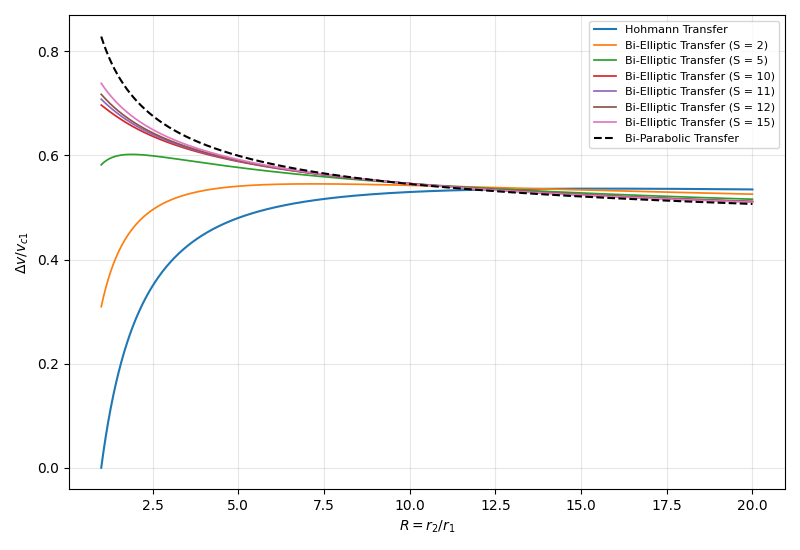
\includegraphics[width=0.85\textwidth]{problem1_full.png}
\caption{Normalized total impulse $\Delta v/v_{c1}$ vs.\ $R=r_2/r_1$ for $R\in[1,20]$.}
\label{fig:p1-full}
\end{figure}

\begin{figure}[H]
\centering
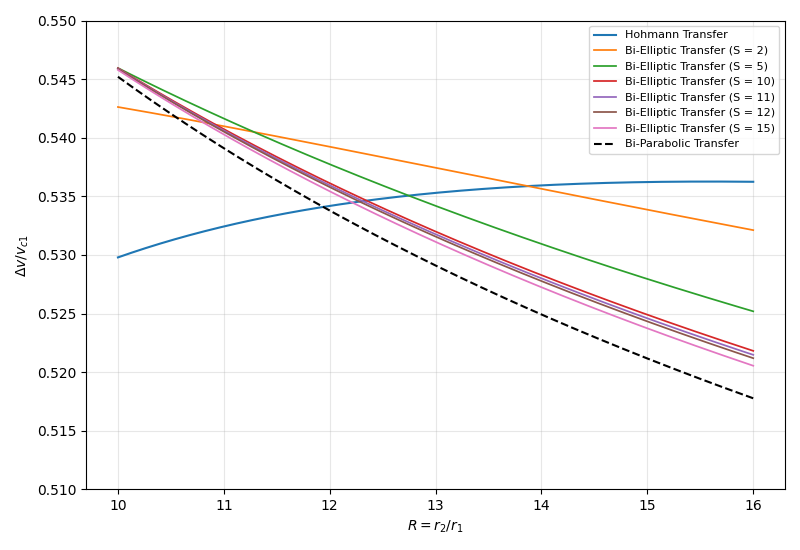
\includegraphics[width=0.85\textwidth]{problem1_zoom.png}
\caption{Enlarged view for $R\in[10,16]$, $\Delta v/v_{c1}\in[0.51,0.55]$.}
\label{fig:p1-zoom}
\end{figure}

\FloatBarrier

\section{Problem 2}
\label{sec:problem2}

The course notes (Section 5.6) state:
\begin{itemize}
  \item $1 < R < 11.94$: the Hohmann transfer is the minimum-impulse transfer.
  \item $R > 11.94$: the bi-parabolic transfer outperforms the Hohmann transfer.
  \item $R > 15.58$: any bi-elliptic transfer with $S > 1$ outperforms the Hohmann transfer.
\end{itemize}

\noindent Using the normalized impulse expressions from Problem 1, \texttt{problem2.py} uses the \texttt{scipy} root-finder \texttt{brentq} to solve the following root-finding problems.

\subsection*{(a) Hohmann vs. bi-parabolic}

The total impulse of each transfer is the sum of its impulses. Summing \eqref{eq:p1-hohmann} and \eqref{eq:p1-biparabolic},
\begin{align*}
\frac{\Delta v_H}{v_{c1}} &= \frac{\Delta v_{1,H}}{v_{c1}} + \frac{\Delta v_{2,H}}{v_{c1}}
  = \sqrt{\frac{2R}{1+R}} - 1 + \sqrt{\frac{1}{R}} - \sqrt{\frac{2}{R(1+R)}}\\[4pt]
\frac{\Delta v_{BP}}{v_{c1}} &= \frac{\Delta v_{1,BP}}{v_{c1}} + \frac{\Delta v_{2,BP}}{v_{c1}}
  = \left(\sqrt{2}-1\right)\left(1+\sqrt{\frac{1}{R}}\right)
\end{align*}
The crossover is the value of $R$ at which the two totals are equal, i.e.\ the root of
\begin{equation}
\boxed{f(R) = \frac{\Delta v_H}{v_{c1}} - \frac{\Delta v_{BP}}{v_{c1}} = 0}
\label{eq:p2-fbp}
\end{equation}
solved with \texttt{brentq} on the bracket $R\in[2,50]$, over which $f$ changes sign.

\subsection*{(b) Hohmann vs. bi-elliptic, for each $S$}

Summing the three impulses of \eqref{eq:p1-bielliptic},
\begin{equation*}
\frac{\Delta v_{BE}}{v_{c1}} = \sqrt{\frac{2RS}{1+RS}} - 1
+ \sqrt{\frac{1}{RS}}\left(\sqrt{\frac{2}{1+S}} - \sqrt{\frac{2}{1+RS}}\right)
+ \sqrt{\frac{2S}{R+RS}} - \sqrt{\frac{1}{R}}
\end{equation*}
For each $S\in\{2,5,10,11,12,15\}$, the crossover is the root of
\begin{equation}
\boxed{g(R;S) = \frac{\Delta v_H}{v_{c1}} - \frac{\Delta v_{BE}}{v_{c1}} = 0}
\label{eq:p2-fbe}
\end{equation}
where $\Delta v_H/v_{c1}$ is the same Hohmann total impulse as shown in part (a). Each root is solved with \texttt{brentq} on the bracket $R\in[2,50]$.

\medskip
\programoutput{outputs/problem2.txt}

\subsection*{(c) Root as a function of $S$}

\begin{figure}[H]
\centering
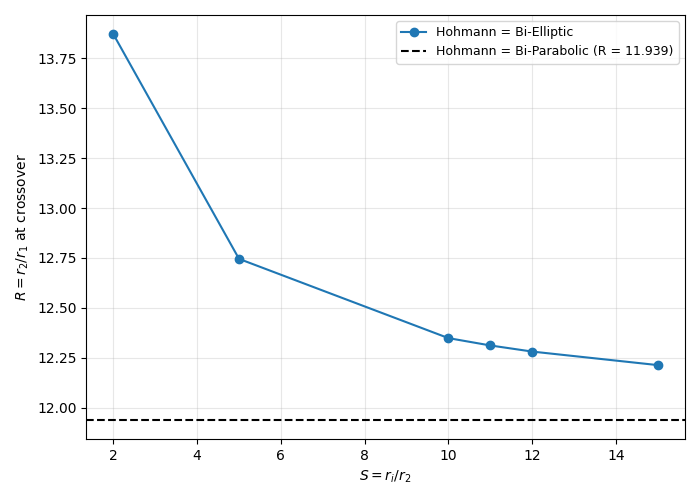
\includegraphics[width=0.75\textwidth]{problem2_roots.png}
\caption{Hohmann/bi-elliptic crossover $R$ vs.\ $S$.}
\label{fig:p2-roots}
\end{figure}

\FloatBarrier

\section{Problem 3}
\label{sec:problem3}

Because the initial and terminal orbits are circular, the radii follow from $v_c=\sqrt{\mu/r}$ with $\mu=1$:
\begin{equation*}
r_1 = \frac{\mu}{v_{c1}^2} = 1, \qquad r_2 = \frac{\mu}{v_{c2}^2} = 4, \qquad R = \frac{r_2}{r_1} = 4
\end{equation*}
The total impulses from Problem 1 are evaluated at $R=4$ in \texttt{problem3.py} (bi-elliptic for $S\in\{2,5,10,11,12,15\}$, as in Problem 1), and the smallest is selected.

\medskip
\programoutput{outputs/problem3.txt}

\begin{equation*}
\boxed{\text{Hohmann transfer}, \qquad \frac{\Delta V}{v_{c1}} = 0.4487}
\end{equation*}

\begin{figure}[H]
\centering
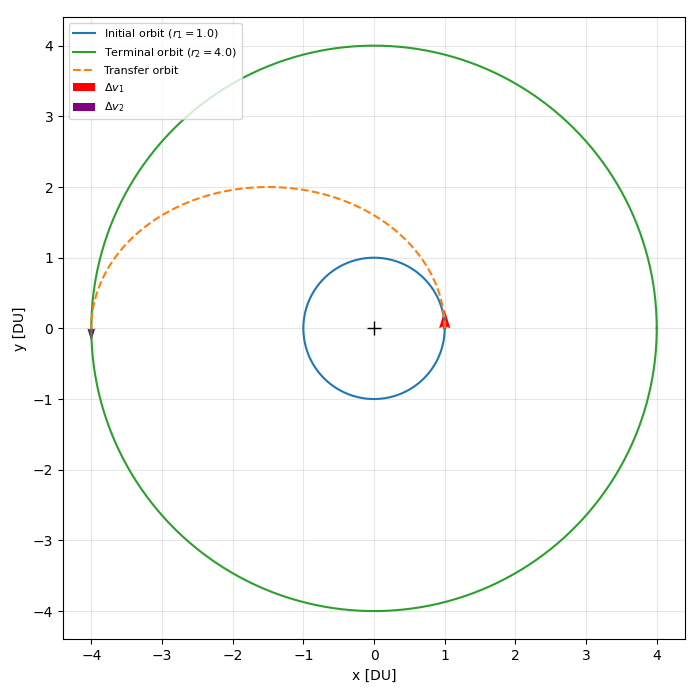
\includegraphics[width=0.65\textwidth]{problem3_transfer.png}
\caption{Hohmann transfer from $r_1=1$ to $r_2=4$ (canonical units), with impulses $\Delta v_1$ and $\Delta v_2$ shown at periapsis and apoapsis of the transfer ellipse.}
\label{fig:p3-transfer}
\end{figure}

\FloatBarrier

\section{Problem 4}
\label{sec:problem4}

The LEO radius follows from the altitude, and the GEO radius from the orbital period (Eq.~1.123 from the course notes):
\begin{equation*}
r_1 = R_E + 300~\text{km} = 6678~\text{km}, \qquad
\tau = 2\pi\sqrt{\frac{r_2^3}{\mu}} \;\Rightarrow\; r_2 = \left(\frac{\mu \tau^2}{4\pi^2}\right)^{1/3}, \qquad
a = \frac{r_1+r_2}{2}
\end{equation*}

\subsection*{(a) and (b) Impulse magnitudes and total $\Delta V$}

The first impulse is tangential (energy change only):
\begin{equation*}
\Delta v_1 = \sqrt{\frac{2\mu}{r_1}-\frac{\mu}{a}} - \sqrt{\frac{\mu}{r_1}}
\end{equation*}
The second impulse circularizes the orbit and rotates the plane by $\theta$ (law of cosines, Eq.~5.53 from the course notes):
\begin{equation*}
\Delta v_2 = \sqrt{(v_2^-)^2 + (v_2^+)^2 - 2v_2^-v_2^+\cos\theta}, \qquad
v_2^- = \sqrt{\frac{2\mu}{r_2}-\frac{\mu}{a}}, \qquad v_2^+ = \sqrt{\frac{\mu}{r_2}}
\end{equation*}
GEO is equatorial ($i_2=0$), so Eq.~5.50 from the course notes gives $\cos\theta = \cos i_1$, i.e.\ $\theta = i_1 = 57^\circ$. The total is
\begin{equation*}
\boxed{\Delta V = \Delta v_1 + \Delta v_2}
\end{equation*}

\subsection*{(c) Time of flight}
Half the period of the transfer orbit:
\begin{equation*}
t_f = \pi\sqrt{\frac{a^3}{\mu}}
\end{equation*}

\subsection*{(d) Mass ratios}
From the rocket equation (Eq.~4.38),
\begin{equation*}
\Delta v = g_0 I_{sp}\ln\left(\frac{m_0}{m_f}\right)
\end{equation*}
so for each impulse
\begin{equation*}
\frac{m_0}{m_f} = \exp\left(\frac{\Delta v_k}{g_0 I_{sp}}\right), \qquad k = 1,2, \qquad I_{sp} = 320~\text{s}
\end{equation*}

\noindent The expressions in parts (a) through (d) are evaluated in \texttt{problem4.py} with $\mu = 398600~\text{km}^3/\text{s}^2$, $R_E = 6378$~km, $\tau = 23.934$~h, $g_0 = 9.80665~\text{m/s}^2$, and $I_{sp} = 320$~s, giving:

\medskip
\programoutput{outputs/problem4.txt}

\subsection*{(e) Hohmann transfer plot}

\begin{figure}[H]
\centering
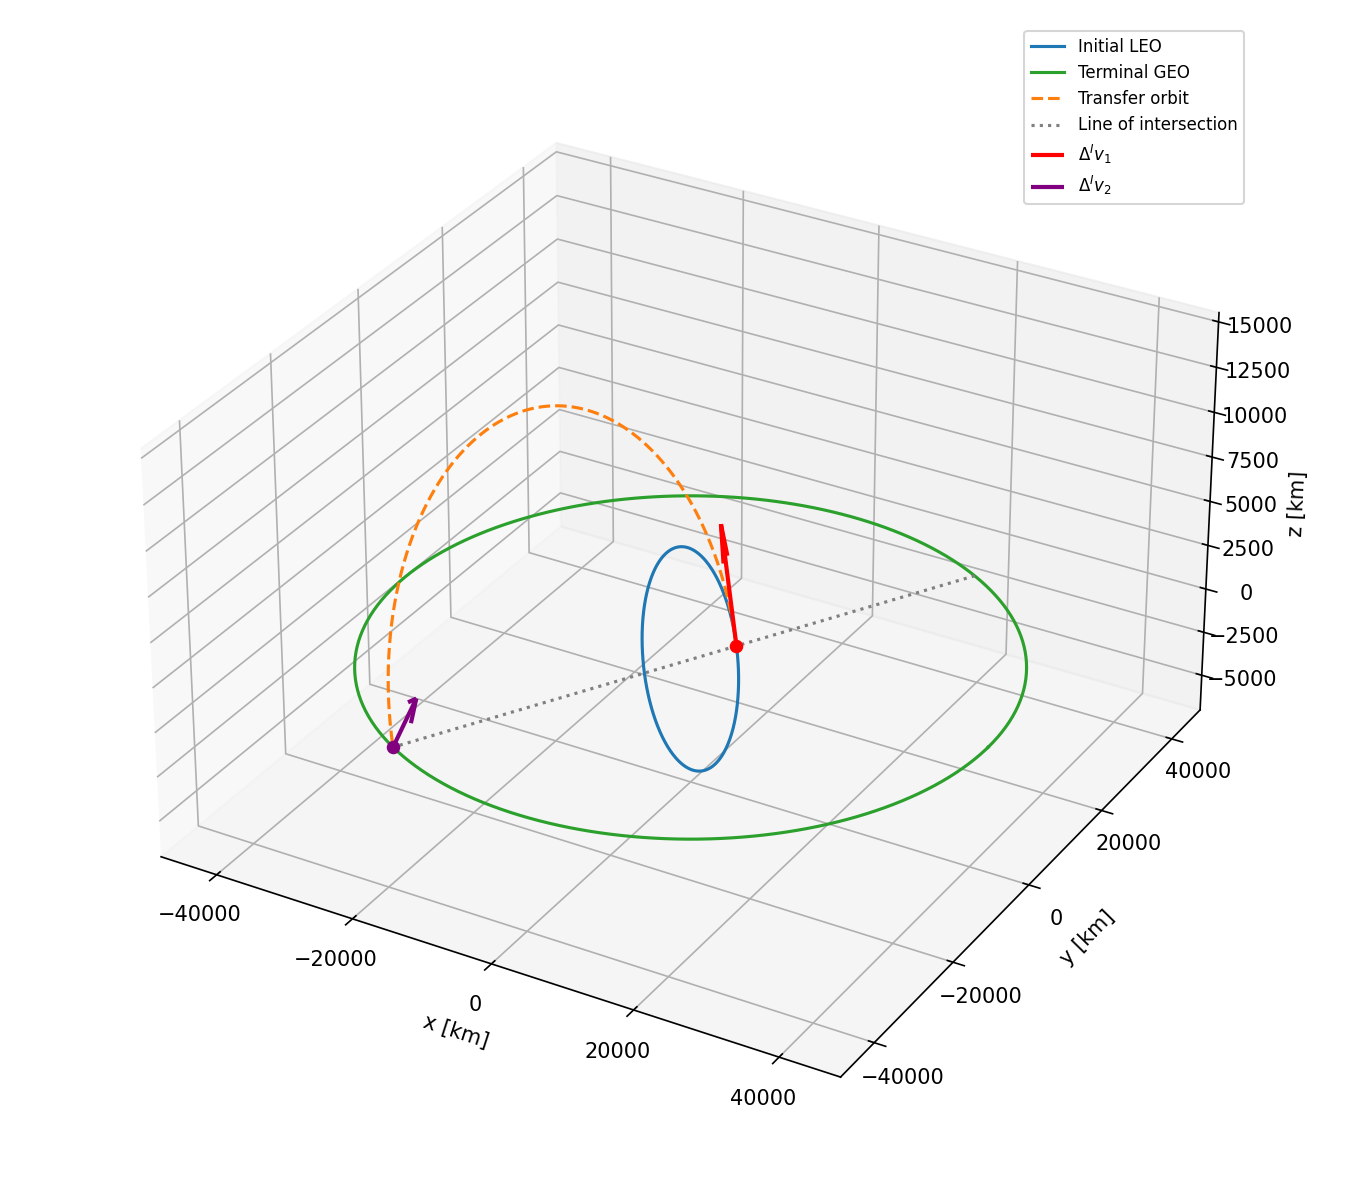
\includegraphics[width=0.8\textwidth]{problem4_transfer.png}
\caption{LEO-to-GEO Hohmann transfer with the plane change at apoapsis.}
\label{fig:p4-transfer}
\end{figure}

\subsection*{(f) Effect of $\Omega$ on the transfer start}

The second impulse must lie on the line of intersection between the initial and terminal orbital planes. Because the terminal orbit is equatorial (GEO), this line of intersection is the line of nodes of the initial orbit. The first impulse is $180^\circ$ away from the second impulse on this same line, so the transfer starts at the opposite node of the initial orbit. Changing $\Omega$ rotates the line of nodes about $\vect{I}_z$, which moves the start point in ECI coordinates, but it is still the node of the initial orbit.
\begin{equation*}
\boxed{\text{No. The transfer always starts at the node of the initial orbit, regardless of }\Omega.}
\end{equation*}

\FloatBarrier

\section{Problem 5}
\label{sec:problem5}

The longitudes of the ascending node are not given, so both orbits can be assumed to have $\Omega_1=\Omega_2=0$. The LEO radius can be found with the altitude:
\begin{equation*}
r_1 = R_E + 350~\text{km} = 6728~\text{km}, \qquad r_2 = 26558~\text{km}, \qquad \Omega_1 = \Omega_2 = 0
\end{equation*}

\subsection*{(a) and (b) Line of intersection and impulse positions}
The angular momentum directions, the line of intersection, and the impulse positions can be found in the course notes:
\begin{equation*}
\hat{\vect{h}}_k = \sin i_k\sin\Omega_k\,\vect{I}_x - \sin i_k\cos\Omega_k\,\vect{I}_y + \cos i_k\,\vect{I}_z
\end{equation*}
\begin{equation*}
\vect{\ell} = \frac{\ivect{h}_1\times\ivect{h}_2}{\|\ivect{h}_1\times\ivect{h}_2\|}
\end{equation*}
\begin{equation*}
\vect{r}_1 = r_1\vect{\ell}, \qquad \vect{r}_2 = -r_2\vect{\ell}
\end{equation*}

\subsection*{(c) Total $\Delta V$}
We can find $\Delta V$ using the transfer orbit semi-major axis and the first and second impulses:
\begin{equation*}
a = \frac{r_1+r_2}{2}
\end{equation*}
\begin{equation*}
\Delta v_1 = \sqrt{\frac{2\mu}{r_1}-\frac{\mu}{a}} - \sqrt{\frac{\mu}{r_1}}
\end{equation*}
\begin{equation*}
\Delta v_2 = \sqrt{(v_2^-)^2 + (v_2^+)^2 - 2v_2^-v_2^+\cos\theta}, \qquad
v_2^- = \sqrt{\frac{2\mu}{r_2}-\frac{\mu}{a}}, \qquad v_2^+ = \sqrt{\frac{\mu}{r_2}}
\end{equation*}
The rotation angle $\theta$ follows from
\begin{equation*}
\cos\theta = \hat{\vect{h}}_1\cdot\hat{\vect{h}}_2
= \sin i_1\sin i_2\left(\sin\Omega_1\sin\Omega_2 + \cos\Omega_1\cos\Omega_2\right) + \cos i_1\cos i_2
\end{equation*}
This reduces to $i_2-i_1$ because $\Omega_1=\Omega_2$:
\begin{align*}
\cos\theta &= \sin i_1\sin i_2\left(\sin^2\Omega_1 + \cos^2\Omega_1\right) + \cos i_1\cos i_2 \\
&= \cos i_1\cos i_2 + \sin i_1\sin i_2 = \cos(i_2-i_1)
\;\Rightarrow\; \theta = i_2 - i_1
\end{align*}
And thus:
\begin{equation*}
\boxed{\Delta V = \Delta v_1 + \Delta v_2
= \sqrt{\frac{2\mu}{r_1}-\frac{\mu}{a}} - \sqrt{\frac{\mu}{r_1}}
+ \sqrt{(v_2^-)^2 + (v_2^+)^2 - 2v_2^-v_2^+\cos(i_2-i_1)}}
\end{equation*}

\subsection*{(d), (e), and (f) Time of flight, eccentricity, and plane rotation angle}
The time of flight is half the transfer orbit's period, eccentricity can be found with the initial and terminal radii, and the rotation angle is $\theta$, given above:
\begin{equation*}
t_f = \pi\sqrt{\frac{a^3}{\mu}}, \qquad
e = \frac{r_2-r_1}{r_2+r_1}
\end{equation*}

\medskip
\noindent The expressions in parts (a) through (f) are evaluated in \texttt{problem5.py} with $\mu = 398600~\text{km}^3/\text{s}^2$ and $R_E = 6378$~km, giving:

\medskip
\programoutput{outputs/problem5.txt}

\subsection*{(g) Transfer plot}

\begin{figure}[H]
\centering
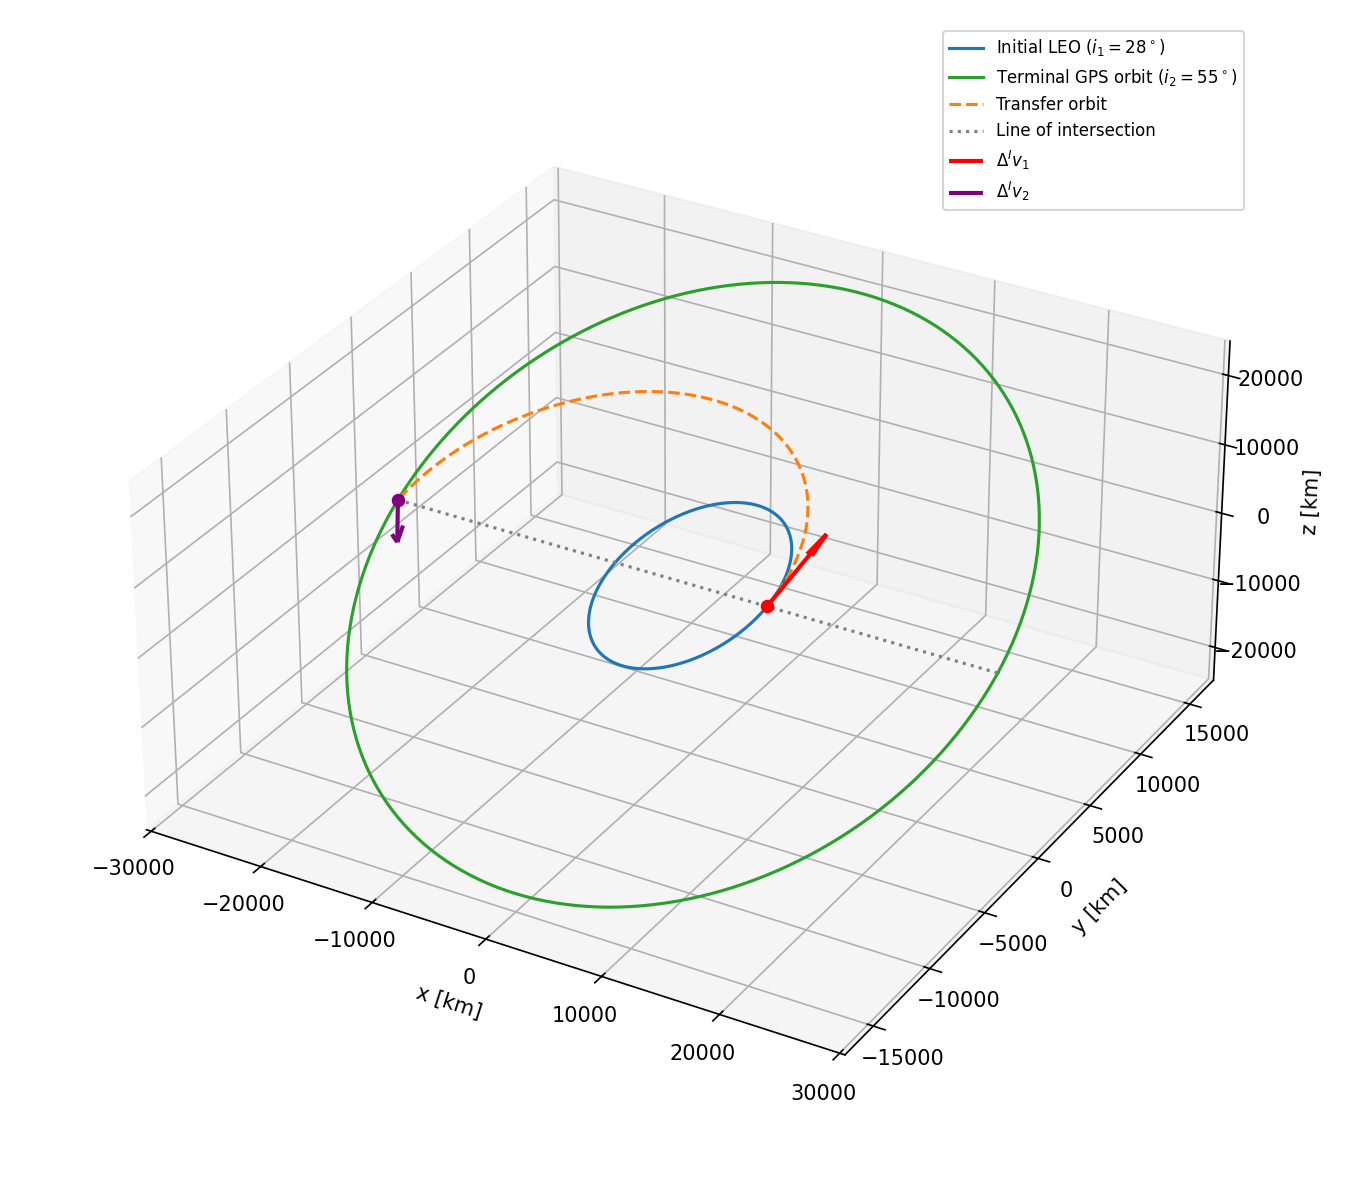
\includegraphics[width=0.8\textwidth]{problem5_transfer.png}
\caption{Two-impulse LEO-to-GPS transfer with both impulses on the line of intersection.}
\label{fig:p5-transfer}
\end{figure}

\FloatBarrier

\section{Problem 6}
\label{sec:problem6}

The LEO radius can be found from the altitude, and the GEO radius can be found from the fact that the period must be $24$~hours:
\begin{equation*}
r_1 = R_E + 300~\text{km} = 6678~\text{km}, \qquad
r_2 = \left(\frac{\mu \tau^2}{4\pi^2}\right)^{1/3}, \qquad
a = \frac{r_1+r_2}{2}
\end{equation*}
The circular speeds and the transfer orbit speeds at periapsis and apoapsis are
\begin{equation*}
v_{c1} = \sqrt{\frac{\mu}{r_1}}, \qquad
v_p = \sqrt{\frac{2\mu}{r_1}-\frac{\mu}{a}}, \qquad
v_a = \sqrt{\frac{2\mu}{r_2}-\frac{\mu}{a}}, \qquad
v_{c2} = \sqrt{\frac{\mu}{r_2}}
\end{equation*}
A fraction $f$ of the inclination change $\Delta i = 28.5^\circ$ is performed with the first impulse and $1-f$ with the second. Each impulse follows from Eq.~5.53:
\begin{equation*}
\Delta v_1(f) = \sqrt{v_{c1}^2 + v_p^2 - 2v_{c1}v_p\cos(f\,\Delta i)}, \qquad
\Delta v_2(f) = \sqrt{v_a^2 + v_{c2}^2 - 2v_a v_{c2}\cos\big((1-f)\,\Delta i\big)}
\end{equation*}
\begin{equation*}
\Delta V(f) = \Delta v_1(f) + \Delta v_2(f)
\end{equation*}

\subsection*{(a) and (b) Total impulse for $f=0$ and $f=1$}
All of the inclination change at apoapsis is $f=0$, and all of it at the initial LEO is $f=1$:
\begin{equation*}
\Delta V_{(a)} = \Delta V(0), \qquad \Delta V_{(b)} = \Delta V(1)
\end{equation*}
\subsection*{(c) Total impulse as a function of $f$}
$\Delta V(f)/v_{c1}$ for $f\in[0,1]$ in increments of $0.01$:

\begin{figure}[H]
\centering
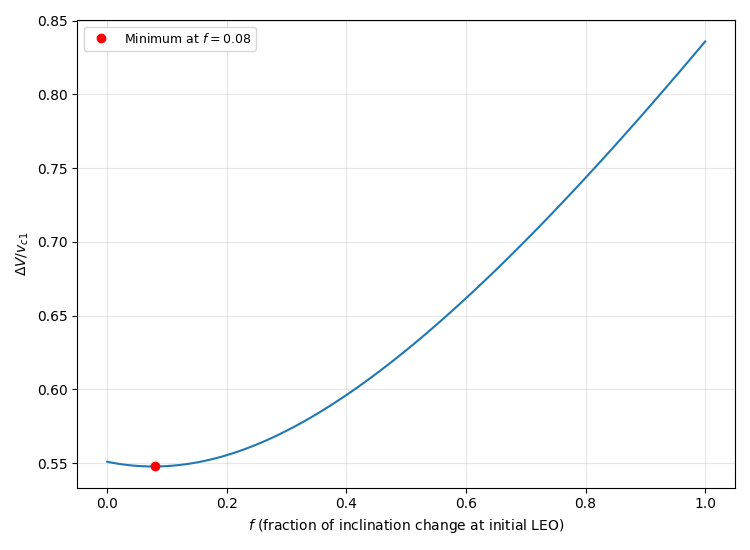
\includegraphics[width=0.65\textwidth]{problem6_dv_vs_f.png}
\caption{Normalized total impulse $\Delta V/v_{c1}$ vs.\ $f$.}
\label{fig:p6-dv}
\end{figure}

\subsection*{(d) Minimum-impulse fraction}
From \Cref{fig:p6-dv}, the smallest total impulse ($\Delta V/v_{c1} = 0.5478$) occurs at
\begin{equation*}
\boxed{f = 0.08}
\end{equation*}

\medskip
\noindent The expressions in parts (a) through (d) are evaluated in \texttt{problem6.py} with $\mu = 398600~\text{km}^3/\text{s}^2$ and $R_E = 6378$~km, giving:

\medskip
\programoutput{outputs/problem6.txt}

\FloatBarrier


\dividerpage{Appendices}{Python Source Code}{All code and sources found in: \repolink}
\appendix
\section{transfers.py}
\lstinputlisting[caption={transfers.py}]{../transfers.py}
\clearpage

\section{orbit\_utils.py}
\lstinputlisting[caption={orbit\_utils.py}]{../orbit_utils.py}
\clearpage

\section{problem1.py}
\lstinputlisting[caption={problem1.py}]{../problem1.py}
\clearpage

\section{problem2.py}
\lstinputlisting[caption={problem2.py}]{../problem2.py}
\clearpage

\section{problem3.py}
\lstinputlisting[caption={problem3.py}]{../problem3.py}
\clearpage

\section{problem4.py}
\lstinputlisting[caption={problem4.py}]{../problem4.py}
\clearpage

\section{problem5.py}
\lstinputlisting[caption={problem5.py}]{../problem5.py}
\clearpage

\section{problem6.py}
\lstinputlisting[caption={problem6.py}]{../problem6.py}


\end{document}
